\section{Weather Model}
As Fig.3 shows, the weather model contains a uniform random number generator, an adder, and a delay. The uniform random number generator is used to simulate raindrops, which generates a sequence of "raindrops" that follows the uniform distribution from 1 ml to 8 ml at each timestamp. The delay stores the volume of remaining water. At each timestamp, the adder adds the newly generated "raindrop" with remaining water and the output is received by the rain sensor model.
\begin{center}
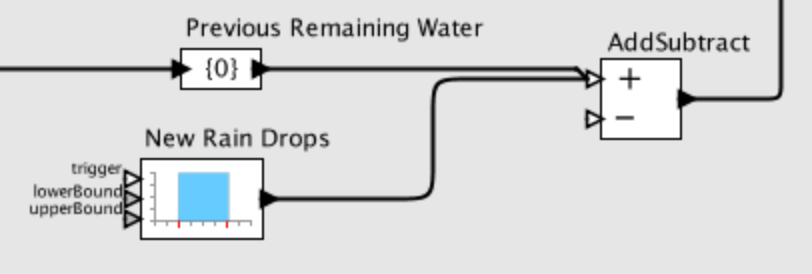
\includegraphics[width=13.5cm]{fig3.png}
\end{center}
\begin{center}
\small{Figure 3. The Weather Model}
\label{weather}
\end{center}